\documentclass[12pt]{article}

\usepackage[margin=1in]{geometry}
\usepackage{setspace}
\usepackage{amsmath, amssymb}
\usepackage{graphicx}
\usepackage{booktabs}
\usepackage{threeparttable}
\usepackage{hyperref}
\usepackage{placeins}

\onehalfspacing

\title{Attribution Framing by Outlet Political Lean: \\ A Companion Analysis}
\author{Hariaksha Gunda}
\date{\today}

\begin{document}
\maketitle

\section*{Purpose}

This memo supplements Section 5.5 (``Variation by Outlet
Characteristics'') of the main paper, \emph{Reading the Storm}. That
section reports a regression of article-level attribution scores on a
continuous outlet political-lean measure (Ad Fontes Bias score). This
memo presents the same relationship visually, as a time trend split by
outlet political lean, and documents why one of the three lean groups
--- Right-leaning outlets --- is represented by only a small number of
articles.

This is a working memo, not a paper section: it is meant to inform a
conversation with the coauthor team about how (or whether) to extend
the outlet-lean data collection, not to be read as a finished result.

\section*{Methodology}

Outlet political lean is determined exactly as in the main paper.
Each article's URL is parsed down to its bare domain (e.g.\
\texttt{nytimes.com}), which is then looked up against Ad Fontes
Media Bias Chart's numeric ``Bias'' score --- a continuous scale from
roughly $-42$ (furthest left) to $+42$ (furthest right) --- for the 33
domains in the sample that Ad Fontes has individually rated. An
article is classified as:

\begin{itemize}
  \item \textbf{Left-leaning} if its domain has a negative Bias score,
  \item \textbf{Right-leaning} if its domain has a positive Bias
    score,
  \item \textbf{Unidentified} if its domain has no individually-rated
    Bias score (either because the domain was never rated, or because
    it was rated but no numeric score was available --- one domain,
    \texttt{al.com}, falls in this category due to a data error on
    Ad Fontes' page for that outlet).
\end{itemize}

These lean labels, along with the underlying numeric Bias score, are
now stored directly as columns on the \texttt{Master} sheet of
\texttt{attribution.xlsx} (\texttt{Domain}, \texttt{Ad Fontes Bias
Score}, \texttt{AllSides Rating (Numeric)}, \texttt{Political Lean
Group}), rather than being computed only at analysis time.

Unlike Figure 1 of the main paper, which plots the disaster-level
Attribution Index (one point per disaster), this analysis plots the
\emph{article}-level attribution score $a_{i,d}$, since outlet lean
only varies at the article level --- the same disaster is frequently
covered by both a left- and a right-leaning outlet, so collapsing to
one number per disaster would discard the variation this chart is
meant to show.

\subsection*{Sample composition}

Table~\ref{tab:lean_counts} shows how the 1,252 Relevant articles
split across the three lean groups.

\begin{table}[h]
\centering
\begin{tabular}{lrr}
\toprule
Group & Articles & Share \\
\midrule
Left-leaning & 869 & 69.4\% \\
Unidentified & 363 & 29.0\% \\
Right-leaning & 20 & 1.6\% \\
\bottomrule
\end{tabular}
\caption{Relevant articles by outlet political-lean group.}
\label{tab:lean_counts}
\end{table}

The Right-leaning group is thin: only 6 of the 33 individually-rated
domains in the sample have a positive Ad Fontes Bias score (Deseret
News, New York Post, OC Register, Boston Herald, Wall Street Journal,
Las Vegas Review-Journal), and together they contribute just 20
articles across the full 2000--2024 sample --- roughly half of them
from Deseret News alone.

\FloatBarrier
\section*{Chart}

Figure~\ref{fig:lean_trend} plots the annual article-level mean
attribution score for Left-leaning and Unidentified outlets
($\pm 1$ SE, with the article count $n$ labeled at each point), and a
binned mean for Right-leaning outlets. Because Right-leaning coverage
is so sparse --- several individual years have zero Right-leaning
articles at all --- an annual mean for that group would mostly be
undefined or based on 1--2 articles. Instead, Right-leaning articles
are pooled into three periods (2000--2019, 2020--2021, 2022--2024),
chosen only to keep each bin's article count usable ($n=5$, $n=9$,
$n=6$ respectively), not because of any hypothesized break at those
specific years.

\begin{figure}[h]
\centering
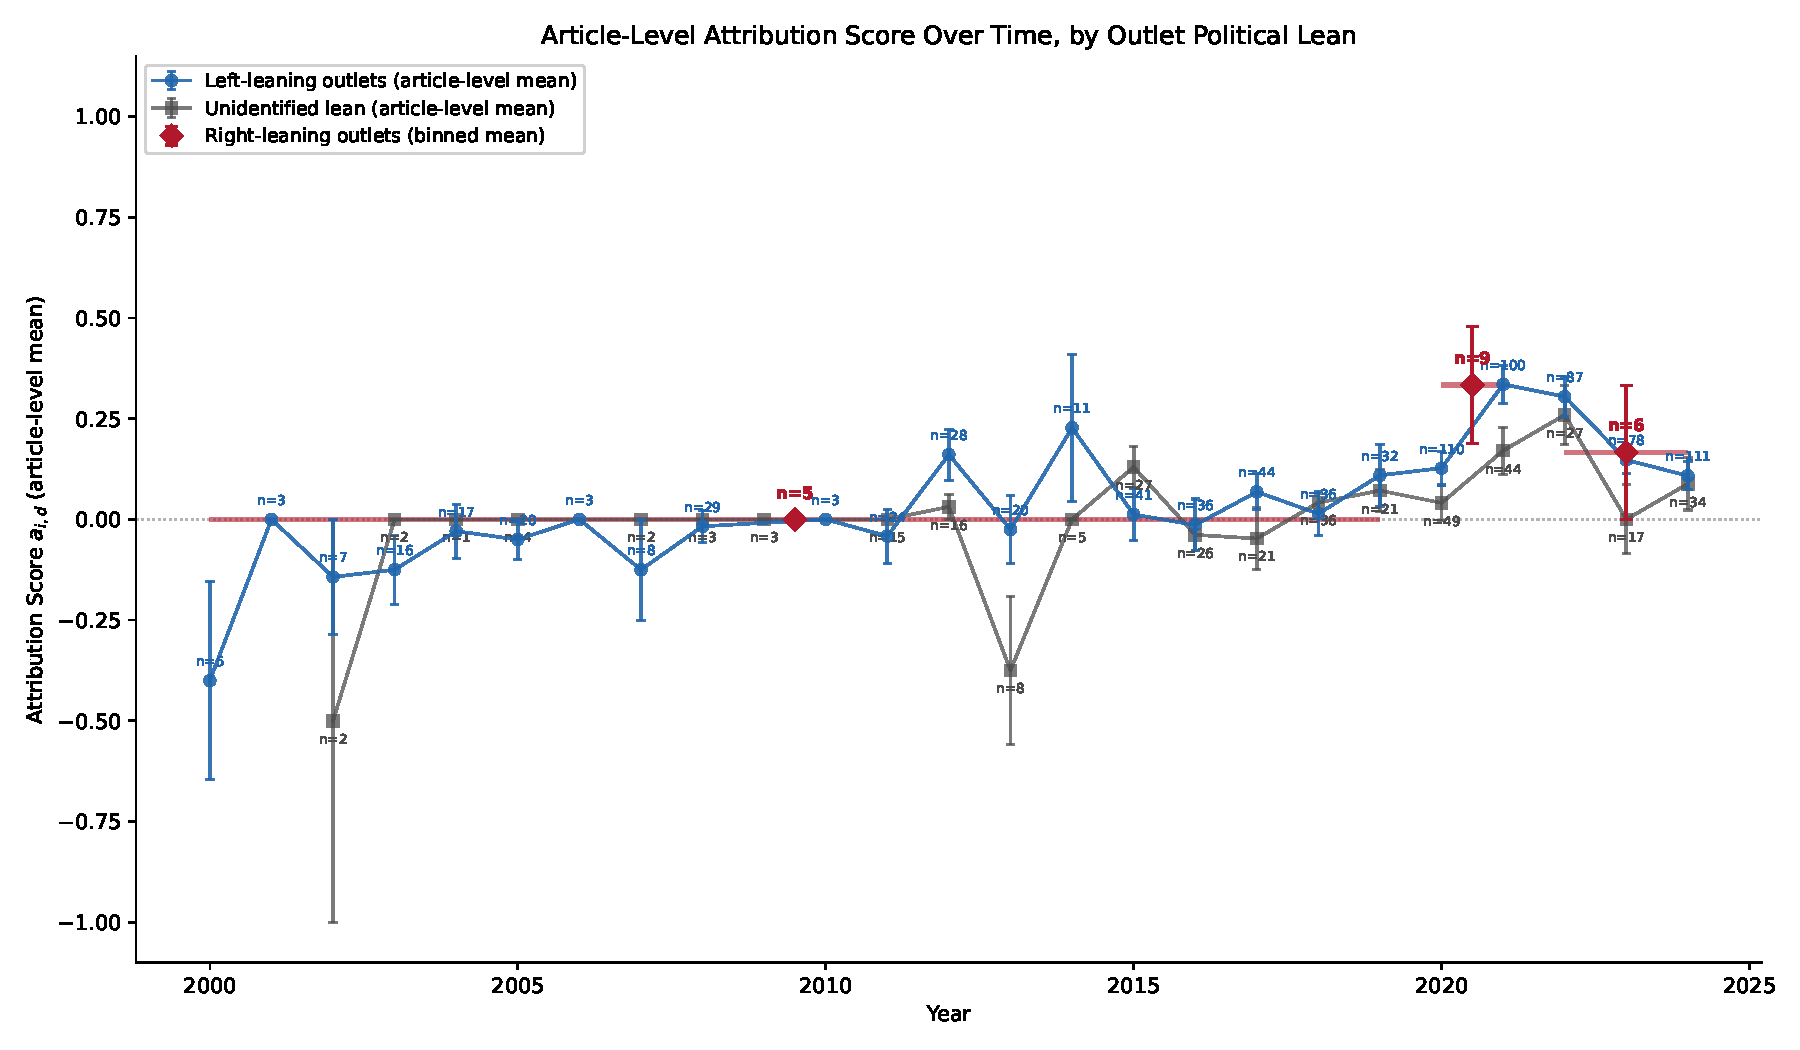
\includegraphics[width=\textwidth]{figures/attribution_by_lean.pdf}
\caption{Article-level attribution score over time, by outlet
political lean. Left-leaning and Unidentified are annual means
($\pm 1$ SE); Right-leaning is a binned mean across three periods
given its small sample.}
\label{fig:lean_trend}
\end{figure}

\FloatBarrier
\subsection*{Reading this chart}

Left-leaning and Unidentified outlets show broadly the same pattern
documented in the main paper's Figure 1: near-zero or negative average
attribution scores through the mid-2000s, rising toward modestly
positive values after 2010, with a further increase from roughly 2020
onward. The Right-leaning group's binned mean is directionally similar
--- near zero pre-2020, rising in the two most recent bins --- but
this should be treated as illustrative rather than statistically
reliable, given the sample sizes involved. The widest error bar in the
figure (the 2020--2021 Right-leaning bin) still rests on only 9
articles.

\section*{Why is Right-leaning representation so thin?}

We investigated whether this imbalance reflects a fixable issue in the
article-retrieval pipeline (\texttt{code/google\_search.py} and
\texttt{code/build\_state\_engine\_mapping.py}) rather than the LLM
coding step. Three findings:

\begin{enumerate}
  \item \textbf{It is not a coding-stage bias.} Candidate articles from
  Right-leaning domains convert to \texttt{Relevant} at a 100\% rate
  (every candidate article retrieved from a Right-leaning domain was
  coded Relevant), actually higher than the 60--92\% conversion rate
  for the largest Left-leaning domains. The LLM relevance-screening
  step is not filtering out Right-leaning content disproportionately
  --- the shortfall happens upstream, at retrieval.

  \item \textbf{Fox News, despite being in the search domain list,
  returned zero candidate articles across all 313 events and 24
  years.} Fox News (\texttt{foxnews.com}) and the Wall Street Journal
  (\texttt{wsj.com}) are both explicitly included in the ``National''
  Programmable Search Engine's domain list, and that engine is queried
  for every single disaster event (confirmed in
  \texttt{build\_state\_engine\_mapping.py}: the National engine is
  added to every event's engine set unconditionally). Yet
  \texttt{foxnews.com} produced 0 candidate articles, and
  \texttt{wsj.com} produced only 1, across the entire sample. The
  likely mechanism: the Google Custom Search API returns only the top
  10 organic results per query, and a single Programmable Search
  Engine spans dozens of domains at once with no live per-domain
  restriction --- so for a given disaster-name query, Google's own
  ranking decides which domains fill those 10 slots. Wire-syndicated
  coverage that gets republished verbatim across the \emph{New York
  Times}, \emph{Washington Post}, CNN, NPR, \emph{USA Today}, and AP
  tends to dominate those slots for exact-phrase disaster-name
  queries, crowding out Fox News' and WSJ's own (differently worded)
  coverage of the same events, even though both are eligible domains
  that get queried every time.

  \item \textbf{The domain list itself under-represents Right-leaning
  outlets.} As confirmed separately, the Access World News database's
  own ``national'' tagging covered fewer than 10 genuinely national
  outlets; the remainder of the 47-domain National PSE list appears to
  have been swept in by a fallback rule (domains with no populated
  ``State'' field defaulting to the National bucket) rather than
  deliberate curation. Well-known Right-leaning national outlets that
  were never AWN-tagged at all --- Breitbart, the Washington Examiner,
  National Review, the Daily Wire, Newsmax, the Daily Caller --- are
  absent from the domain list entirely, so they were never eligible to
  be retrieved in the first place. No script currently in
  \texttt{code/} generates \texttt{data/pse\_domains.json}; it appears
  to be a static artifact from earlier in the project rather than a
  reproducible output.
\end{enumerate}

\section*{Possible next step}

If the coauthor team wants better Right-leaning representation, the
most direct fix is a dedicated Programmable Search Engine restricted
to a curated list of Right-leaning national outlets (e.g.\ Fox News,
WSJ, New York Post, Washington Examiner, National Review, the Daily
Wire, Newsmax, the Daily Caller, Breitbart, Washington Times), so those
outlets compete against each other for search-result slots rather than
against \emph{The New York Times} and \emph{Washington Post}. This
would require:

\begin{itemize}
  \item Creating a new Google Programmable Search Engine (a manual
  step in Google's console --- not something that can be done from the
  existing codebase) restricted to the agreed domain list;
  \item Re-running the existing collection pipeline
  (\texttt{google\_search.py}) against just that engine across all 313
  events;
  \item Coding the resulting candidates through the existing LLM
  pipeline (\texttt{llm\_coder.py}) for consistency with the rest of
  the corpus;
  \item Deciding, as a team, how to treat the addition methodologically
  --- since it would mean the Right-leaning subsample was collected
  differently (targeted rather than incidental) from the rest of the
  corpus, which is worth flagging explicitly if it ends up in the
  paper.
\end{itemize}

This memo does not take a position on whether that extension is worth
doing; it is meant to give the team the diagnostic information needed
to decide.

\end{document}
